\section{Action Suggestion}
Action suggestion is a special feature of this software package. The goal is to demonstrate how probabilistic Machine Learning can be used in the User Interface stack of a variety of applications. To demonstrate this, we modelled user actions with elements of probability distributions to infer the next possible action of the user; the model is then updated according to the past experiences that are observed. A suggested action is shown in a separate dock widget on the left side of the screen, and as discussed earlier the user can move them to another position on the screen if desired. Mathematical derivation of the model is not described here but can be found in the appendix.

\begin{figure}[h]
\centering
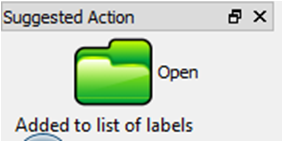
\includegraphics[width=6cm]{after_save_suggestion.png}
\caption{The suggested action is displayed in a dock widget to the left of the user interface}
\label{fig:fullView}
\end{figure}

To build this model we made some assumptions about user actions:
\begin{itemize}
\item Next action of the user only depends on its previous action.
\item Number of possible actions are limited and discrete.
\end{itemize}
These assumptions are made to make the model simpler and possible to implement and test within the time limits of this assignment. We assume the user has four actions: {\textit{Add}, \textit{Delete}, \textit{Open}, and \textit{Save}}. Also the program is preloaded with some prior information about user behaviour after each action. Prior information can be found in table \ref{tab:priors}. This table can be interpreted as the number of times users have chosen a specific action after the action specified in the first column is observed.
\begin{table}[h]
\centering
\begin{tabular}{|c|c|c|c|c|}
\hline \rule[-1ex]{0pt}{3.5ex}  & OPEN & SAVE & EDIT & ADD \\ 
\hline \rule[-1ex]{0pt}{3.5ex} OPEN & 1 & 1 & 3 & 5 \\ 
\hline \rule[-1ex]{0pt}{3.5ex} SAVE & 4 & 1 & 2 & 3 \\ 
\hline \rule[-1ex]{0pt}{3.5ex} EDIT & 0 & 3 & 4 & 3 \\ 
\hline \rule[-1ex]{0pt}{3.5ex} ADD & 1 & 3 & 3 & 3 \\ 
\hline 
\end{tabular}
\caption{priors used for each action}
\label{tab:priors}
\end{table}

Once the program is loaded and the user starts loading images and annotating them their actions will be learnt and used for the next suggestions. For example, if a user opens an image after a new annotation, probability of suggesting that action is increased in later itterations.



Even though no empirical experiment was conducted certain patterns can be observed from a users behaviour which this model can capture. An example of such patterns can be seen when a user saves a file and then opens an image, or when a new image is loaded.  The user then usually starts adding labels to the loaded image. Both of these patterns are produced by the implemented inference system and suggestions are made according to action of the user.
This feature, however, cannot capture all possible patterns, for example it may not be able to suggest reasonable actions after the user has added a new label. This pattern may be modelled if the number of consecutive additions are taken into account. This and many other examples require more sophisticated mathematical models which are not present in this project.
